\documentclass{article}
\usepackage{graphicx}
\usepackage{amsmath}
\usepackage{amssymb}
\usepackage{natbib}

\author{Simon R. Podsiadlik}
\title{Data Analysis: Battery Discharge}
\date{April 30, 2023}

\begin{document}
\maketitle

\section{Abstract}
For this project, we chose to analyze voltage and current data of a discharging 9-Volt battery that we had gathered from the Microcontrollers course. We first plotted the data to physically see the discharge and compare it to what we expected. Then, we used the data to find the overall capacity of an average 9-Volt battery.

\section{Introduction}
The primary objective of this experiment was to measure the discharge of a 9V battery and use that data to determine its overall capacity. To do this, we used an audio-to-digital converter connected to a voltage divider to read the data into a Raspberry Pi. We took voltage and current measurements every five minutes until the battery was no longer in a usable range (lower than 4.8 Volts). Then, we plotted it on a scatter plot. Additionally, we used our current data and integrated it to find the overall capacity of the battery.

\section{Data Collection}
To obtain our data, we built a digital voltmeter circuit using a Raspberry Pi 3 in conjunction with an analog-to-digital converter chip (specifically an ADC0831 chip) and a voltage divider to measure the voltage output over time of a battery. 
The main reason that we needed a voltage divider was because the voltage from the battery exceeded the 5.23V capacity of the ADC chip. \cite{ADC0831} Therefore, we wanted to use a voltage divider to reduce it to about half, and we could determine the necessary resistor values using the voltage divider equation below.

\begin{equation}
    V = V_o \frac{R_1}{R_2 + R_1}
    \label{eq:volt_divide}
\end{equation}

By looking at Equation \ref{eq:volt_divide}, we can determine that if we use two resistors of the same values (for example, 100 Ohms), then our ADC chip would read a range from 0 to 4.5V. Additionally, by choosing two 100 Ohm resistors, our current draw would be about 45 mA, which we can find using Ohm’s law ($\ {V}={I}{R} $). Therefore, since we know that the current draw is 45 mA, and the battery capacity is 400 milliAmp-hours, we can find that the battery should take around 9 hours to discharge. \cite{datasheet}
Lastly, we wanted to find the total charge delivered over time, so we took advantage of the fact that current is the rate of change of charge over time (${I} = \frac{dQ}{dt}$). Therefore, since we would need to integrate to find the charge, we will use right Reimann sums by taking the later point in time. Then we will add each of the sums together to find the overall charge delivered over time.


\section{Visualization}
\begin{figure}[h]
    \centering
    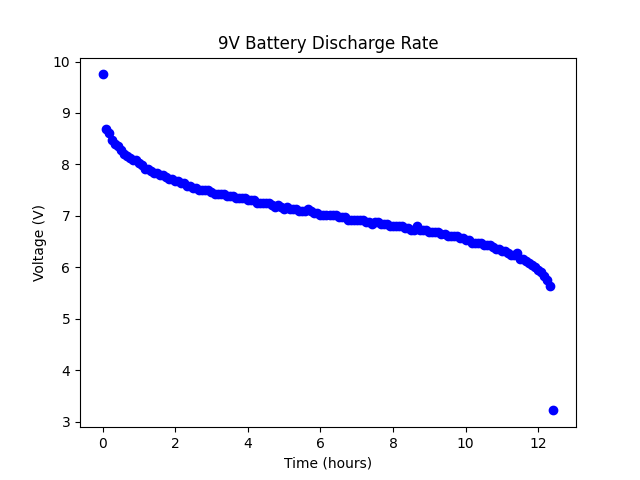
\includegraphics[width=0.5\textwidth]{FinalBatteryDischarge.png}
    \caption{This is the change in voltage for a 9V battery.}
    \label{fig:voltdrop1}
\end{figure}

For this project, we used the matplotlib Python library to plot our voltage and time data onto a graph. As we can see from Figure \ref{fig:voltdrop1}, the battery experiences steep voltage drops at the beginning and end of the overall cycle with a smooth and gradual decay in the middle. Therefore, we can determine that the battery spends most of its time providing outputting between 6 and 8 Volts. If I were to redo these measurements, I would take more data points toward the outer edges to have a more concise reading of the swift voltage drops.

\begin{figure}[h]
    \centering
    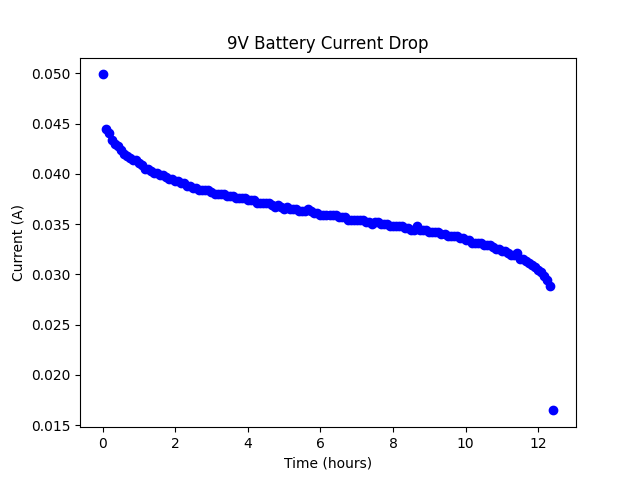
\includegraphics[width=0.5\textwidth]{CurrentDischarge.png}
    \caption{This is the current drop for a 9V battery.}
    \label{fig:currdischarge}

\end{figure}

Next, we used a similar code to plot our current and time data, and we found that the resulting graph (as shown in Figure \ref{fig:currdischarge}) was reminiscent of the voltage graph. In particular, the shape of the slope was exactly the same, with the only difference being the units on the y-axis. This accentuates the relationship between the current and voltage in the discharging battery.

\pagebreak
\section{Results}
First, we wanted to compare our graphs to what we would expect to see. One major point worth noting is that Figure \ref{fig:voltdrop1} is directly related to Figure \ref{fig:currdischarge} by Ohm’s law, which is proved by the graphs being the same shape and being proportional by a factor of 200 (the resistance). Additionally, we can tell that the battery took slightly longer to discharge than we expected, with it taking twelve hours rather than nine.
In the end, we found that the total amount of charge delivered by that battery was 1610.4 Coulombs. Therefore, the capacity, or the total amount of charge initially stored in the battery, is the same value since charge must be conserved. Lastly, since Coulombs are a measure of current and time (Ampere-seconds), we can convert it to milliAmp-hours. When we do this, we found that the capacity is 447.3 milliAmp-hours, which is extremely close to the 450-mA-hr value shown on the data sheet for a 50 mA current draw. \cite{datasheet} Therefore, we can determine that our experiment was a success since the battery readings corroborated the expected values.

\bibliographystyle{plain}
\bibliography{refs}

\end{document}
